\documentclass[12pt,a4paper]{beamer}
\usepackage[utf8]{inputenc}
\usepackage[german]{babel}
\usepackage{amsmath}
\usepackage{amsfonts}
\usepackage{amssymb}
\usepackage{xcolor}
\usepackage{listings}
\usepackage{textcomp}
\usepackage{dirtree}
\usepackage{dialogue}

\definecolor{shadecolor}{RGB}{0,0,0}
\definecolor{textcolor}{RGB}{255,255,255}
\definecolor{bggrey}{RGB}{63,63,63}
\definecolor{simpsongreen}{RGB}{0,85,30}

% Define a Macro to create Image Overlays
\newcommand{\mybox}[1]{\par\noindent\colorbox{shadecolor}
{\color{textcolor}\parbox{\dimexpr\textwidth-2\fboxsep\relax}{\fontsize{3em}{3.5em}\selectfont\textbf{{#1}}}}}

\lstset{
    frame=single,
    breaklines=true,
    postbreak=\raisebox{0ex}[0ex][0ex]{\ensuremath{\color{red}\hookrightarrow\space}},
    basicstyle=\ttfamily\smaller,
    showspaces=false,
    showtabs=false,
    numbersep=5pt, 
    numberstyle=\tiny\color{mygray},
    commentstyle=\color{green!80!red},
    rulecolor=\color{black},
}

\lstdefinestyle{customjava}{
	language=java,
	stringstyle=\color{orange},
	identifierstyle=\color{blue},
}

% Command to remove numbering from footnotes
\newcommand\blfootnote[1]{%
  \begingroup
  \renewcommand\thefootnote{}\footnote{#1}%
  \addtocounter{footnote}{-1}%
  \endgroup
}


\usepackage{tikz}
\usetheme{CambridgeUS}
\setbeamertemplate{navigation symbols}{}%remove navigation symbols

% Presentation Metadata
\author{Sebastian Bachmann \& Tibor Éliás}
\title{How we hacked Online Banking Malware}
\date{22. November 2014}

\begin{document}

\begin{frame}
    \maketitle
    \centering
    B-Sides Vienna
\end{frame}


\section{About Us}
\begin{frame}
	\frametitle{About: Sebastian Bachmann \& Tibor Éliás}
	\begin{itemize}
		\item Mobile Malware Analyst at IKARUS since 2012 / 2013
		\item Analyse Android Malware
		\item Research
		\item Create PoCs
		\item Analysis of Incidents
	\end{itemize}
\end{frame}

\section{About this talk}
\begin{frame}
	\frametitle{What is this all about?}
	\begin{enumerate}
	
		\item Customer Incident: Online Banking Fraud
		\item How we totally f*d up analysis
		\item How we recovered
		\item ... and of course: what we learned!
	\end{enumerate}
\end{frame}


\section{First Analysis}

\begin{frame}
	\frametitle{The incident}
	
	\begin{itemize}
		\item April 2014
		\item Online Banking Trojan detected on PC
		\item Suspicion of mobile component used
		\item Samsung Galaxy Nexus (i9250), Android 4.1
		\item Friday afternoon
	\end{itemize}

\end{frame}

\begin{frame}
\frametitle{Start the Analysis}
\begin{itemize}
	\item[\textbf{\color{green}+}] ADB not enabled
	\item[\textbf{\color{green}+}] Device is not rooted
	\item[\textbf{\color{black}\texttildelow}] No suspicious App icons shown
	\item[\textbf{\color{red}--}] Unknown sources enabled 
	\item[\textbf{\color{red}--}] App lists shows a suspicious app
	\item[\textbf{\color{red}--}] We already knew that the device was compromised
\end{itemize}

\blfootnote{
\textbf{\color{green}+} speak against malware\qquad \textbf{\color{black}\texttildelow} no rating\qquad \textbf{\color{red}--} malware indicator
}
\end{frame}

\begin{frame}[fragile]
	\frametitle{Next steps}
	
	\begin{itemize}
		\item Enable ADB
		\item Pull all installed APKs from device
	
	\begin{lstlisting}[language=bash]
	for app in $(adb shell pm list packages -f | cut -d ':' -f 2 | cut -d '=' -f 1); do 
	DIR=$(dirname $app | tr '/' '_'); 
	[[ ! -d $DIR ]] && mkdir $DIR; 
	adb pull $app $DIR/; done
	\end{lstlisting}

	\item found suspicious \texttt{com.certificate-1.apk}
	\end{itemize}	
\end{frame}

\newcommand{\certificateIcon}{
\includegraphics[keepaspectratio=true,height=0.8cm]{images/icon.png} \texttt{com.certificate-1.apk}}

\begin{frame}
\frametitle{\certificateIcon}
	
	\begin{itemize}
		\item MD5: \texttt{a10fae2ad515b4b76ad950ea5ef76f72}
		\item Package Name: \texttt{com.certificate}
		\item Two Activities
		\item One Service
		\item Three Receivers
		\item 15+ positive results on VirusTotal
		\item Already known as ,,Hesperbot'' \footnote{PC Component Analysis: \url{http://www.welivesecurity.com/wp-content/uploads/2013/09/Hesperbot\_Whitepaper.pdf}}
	\end{itemize}

\end{frame}

\begin{frame}

\frametitle{\certificateIcon}
\resizebox{0.8\textwidth}{0.4\textheight}{
\parbox{\textwidth}{
\dirtree{%
.1 com.certificate-1.apk. 
.2 META-INF. 
.3 CERT.SF. 
.3 MANIFEST.MF. 
.3 CERT.RSA. 
.2 resources.asrc. 
.2 classes.dex\DTcomment{Dalvik Executeable}. 
.2 AndroidManifest.xml. 
.2 assets. 
.3 spy.db\DTcomment{SQLite Database}. 
.2 res. 
.3 xml. 
.4 device\_admin\_policies.xml. 
.3 layout. 
.4 main.xml\DTcomment{Layout File for MainActivity}. 
.3 drawable. 
.4 icon.png. 
}% End dirtree
}
}
\end{frame}


\begin{frame}
\frametitle{\certificateIcon}
	\begin{itemize}
\item android.permission.SEND\_SMS
\item android.permission.INTERNET
\item android.permission.RECEIVE\_WAP\_PUSH
\item android.permission.WRITE\_SMS
\item android.permission.PROCESS\_OUTGOING\_CALLS
\item android.permission.GET\_TASKS
\item android.permission.RECEIVE\_SMS
\item android.permission.READ\_CONTACTS
\item android.permission.RECEIVE\_MMS
\item android.permission.WRITE\_EXTERNAL\_STORAGE
\item android.permission.READ\_SMS
\item android.permission.READ\_LOGS
\item android.permission.RECEIVE\_BOOT\_COMPLETED
\item android.permission.KILL\_BACKGROUND\_PROCESSES
	\end{itemize}
\end{frame}


{
\usebackgroundtemplate{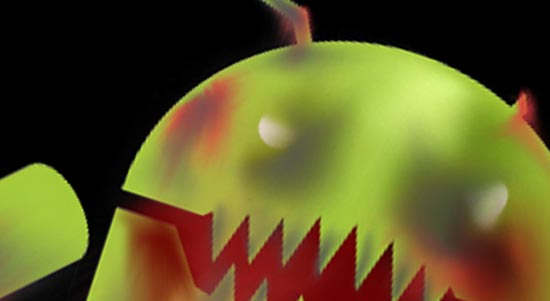
\includegraphics[height=\paperheight]{images/androidmalware.jpg}}
\begin{frame}[plain]

\raisebox{-10em}{\mybox{Malware found...}}
\blfootnote{\color{white}Image (CC BY 2.0) from: \url{https://flic.kr/p/cuZZUY}}
\end{frame}
}


\section{How we f*d up}

\begin{frame}
\frametitle{Meanwhile...}
\begin{dialogue}
\speak{Sebastian} Okay, weekend starts soon so I better remove that thing from the device so we can send it back...

\speak{Tibor} I will start analysis of the sample then and write the report.

\speak{Sebastian} Do you need anything from the device before I remove the malware?

\speak{Tibor} I don't think so...
\end{dialogue}
\end{frame}


\begin{frame}
\frametitle{Removal...}
\textit{Live Demo here... hopefully}
\end{frame}




\section{Shock!}
\begin{frame}
	\frametitle{Meanwhile...}
	\begin{dialogue}
	\speak{Sebastian} Ahh what?
	\speak{Tibor} What was that?
	\speak{Sebastian} I don't know... What was the device PIN again? \direct{tries the PIN...}
	\speak{Tibor} Looks like you just locked the device!
	\speak{Sebastian} Uh oh...
	\end{dialogue}
\end{frame}

{
\usebackgroundtemplate{
\includegraphics[height=\paperheight]{images/fuuu.jpg}}
\begin{frame}[plain]
%\mybox{FFFFFUUUUU!!!}
\end{frame}
}

\section{Revere Engineering}

\begin{frame}[fragile]
\frametitle{A closer look at the Malware}
What's happening on DeviceAdmin onDisableRequest?

\begin{lstlisting}[style=customjava]
if (com.certificate.Cache.getInstance().isContainsSetting("rCode")) {
  String v14 = com.certificate.Util.EncodeThis("uninstall").replace(" ", "");
  v13 = v14.substring(0, (v14.length() - 1));
}
Object v3 = p9.getSystemService("device_policy");
if ((com.certificate.ModuleAdminReceiver.IS_SELF_DEACTIVATION) && (v13.length() > 0)) {
  v3.resetPassword(v13, 0);
  com.certificate.ModuleAdminReceiver.IS_UNINSTALLING = 1;
  v3.lockNow();
}
\end{lstlisting}

\end{frame}

\begin{frame}
\frametitle{A closer look at the Malware}

\begin{itemize}
	\item \texttt{EncodeThis} uses RC5\\
	Blocksize 32bit, Cipher Length 64bit and 12 Rounds
	\item The Cipher is initialised from \texttt{rCode}
	\item \texttt{rCode} (=Response Code) is set on Malware Activation
\end{itemize}

\end{frame}


\begin{frame}
\frametitle{A closer look at the Malware}

\centering
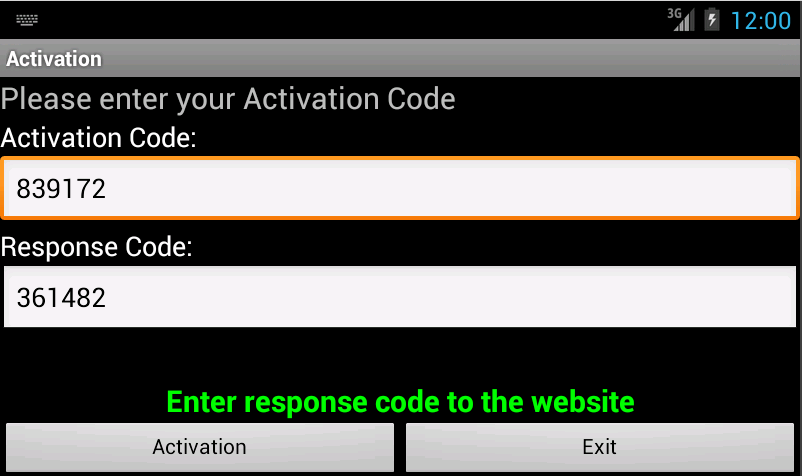
\includegraphics[height=0.6\textheight]{images/activation.png}
\end{frame}

\begin{frame}
\frametitle{Response Code Generation}
\centering
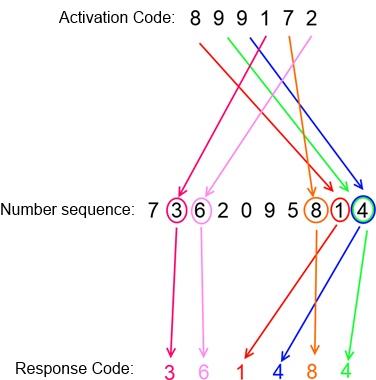
\includegraphics[height=0.8\textheight]{images/code_generation.png}
\end{frame}

\begin{frame}

\mybox{Activiation Code\\is unknown...}
\newline
\newline
... and there is no chance to get it from anywhere

\end{frame}

{
\usebackgroundtemplate{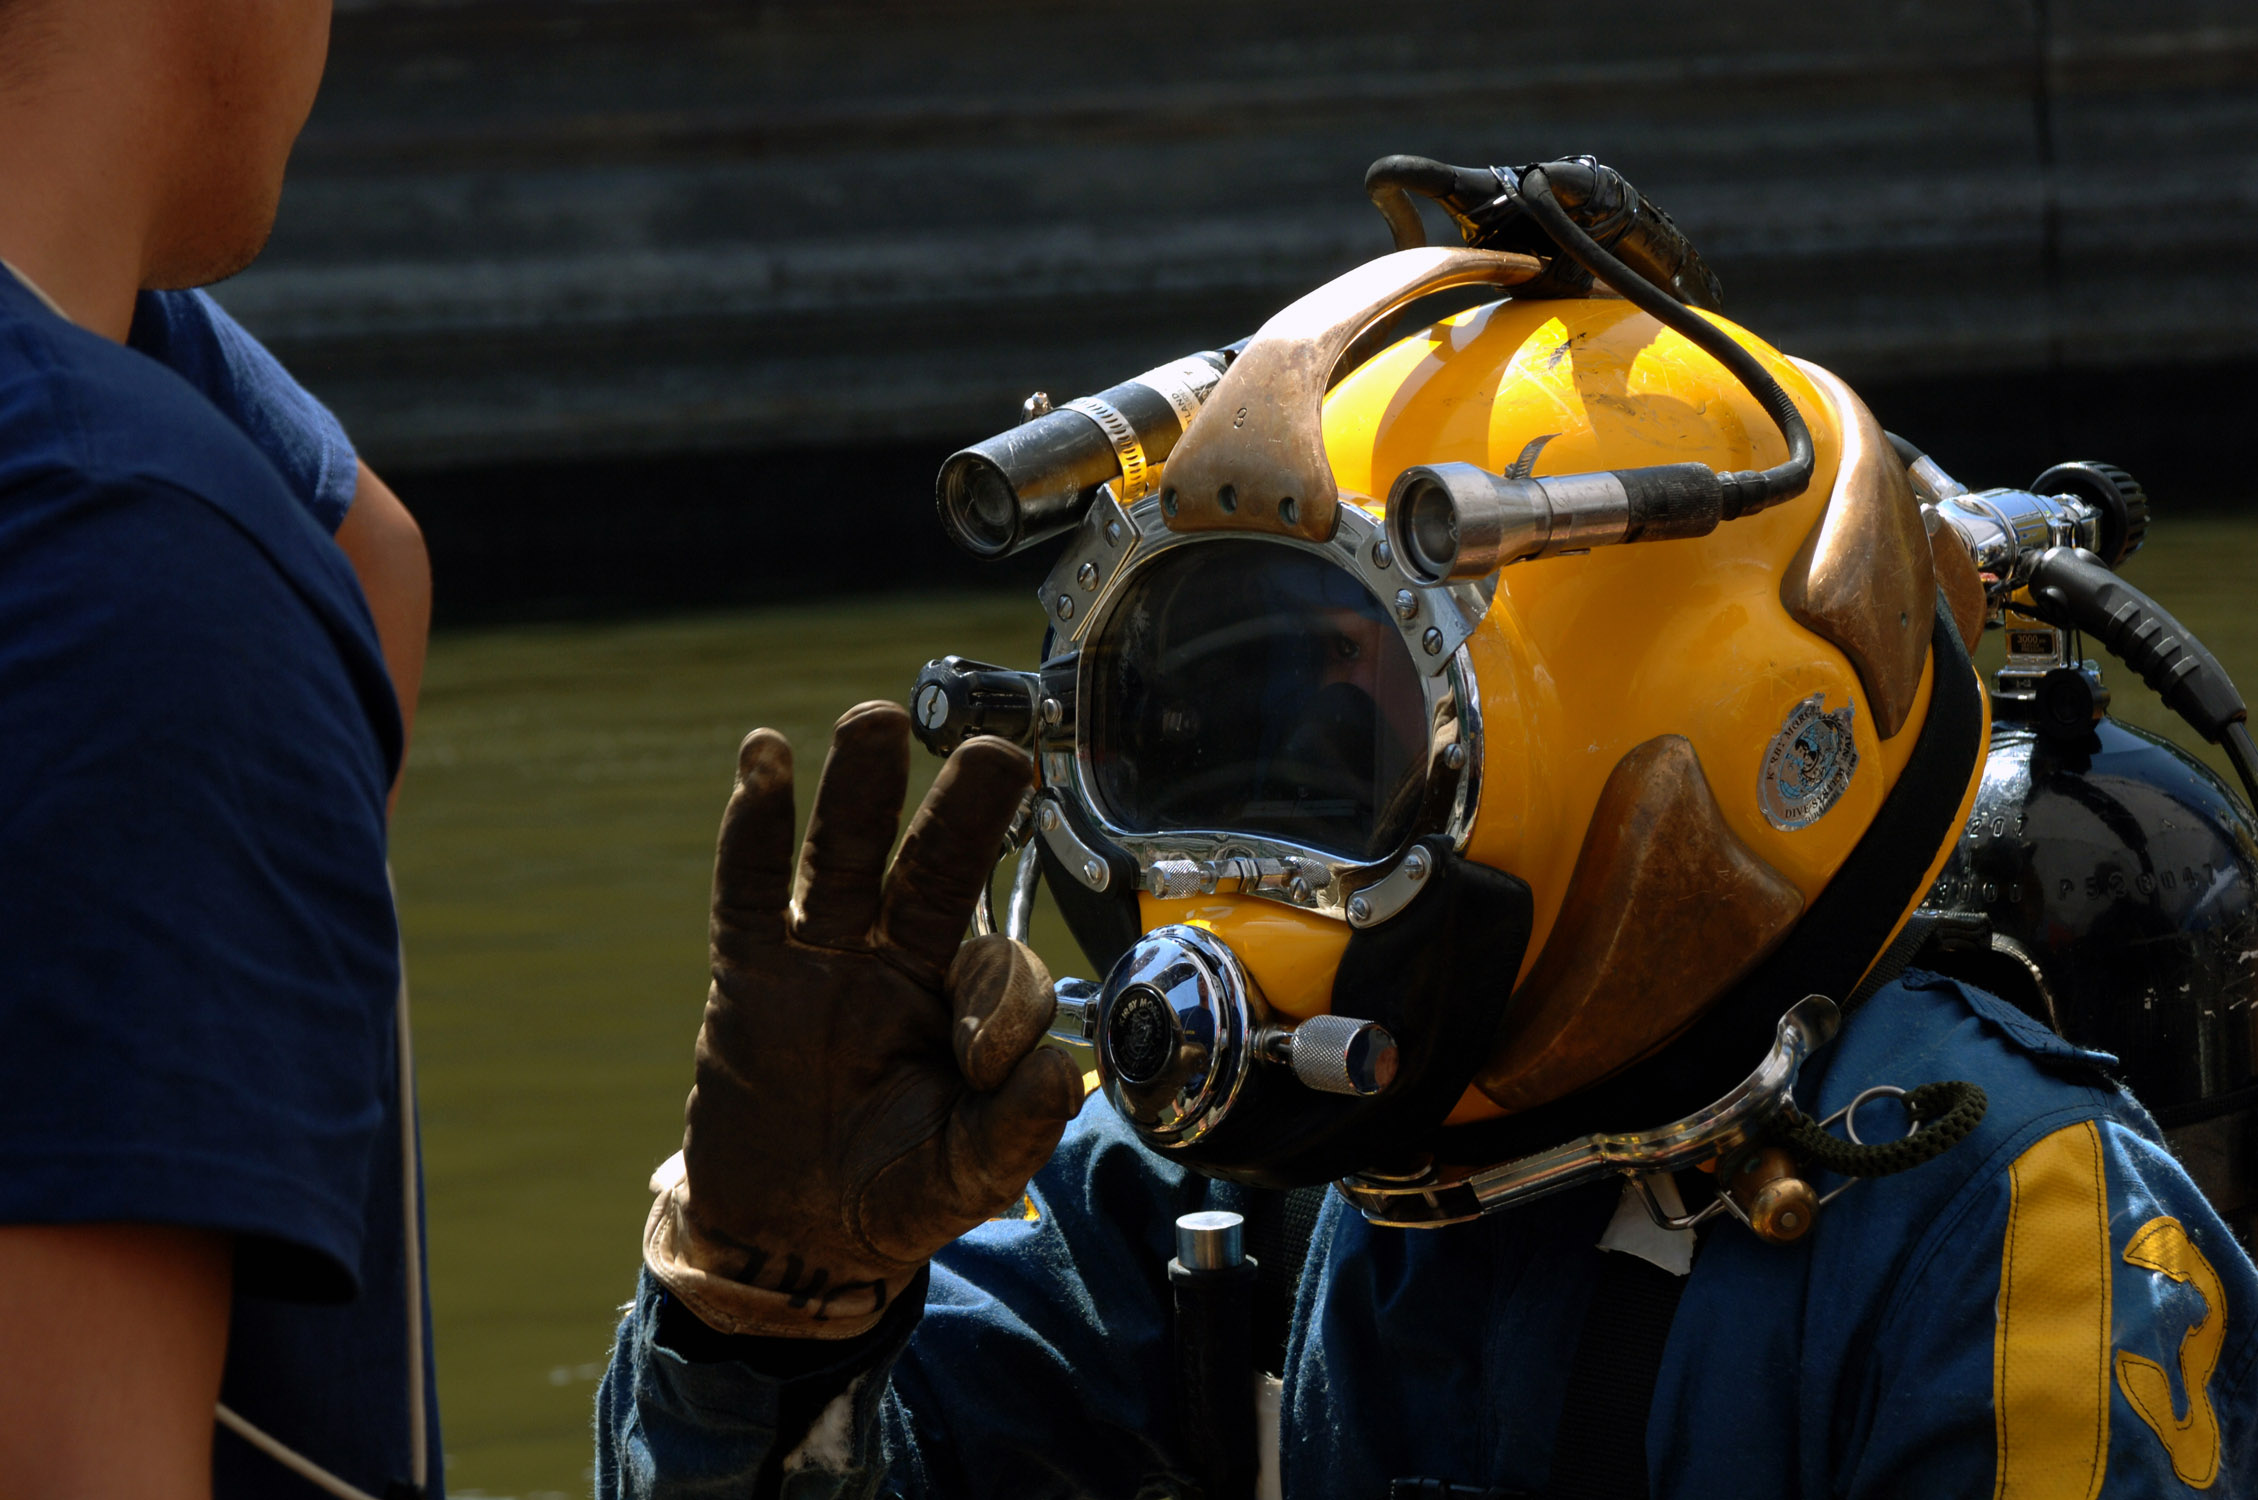
\includegraphics[height=\paperheight]{images/deeper.jpg}}
\begin{frame}[plain]
\raisebox{16em}{\mybox{We need\\to go deeper}}

\blfootnote{\color{white}Image (CC-PD) from: \url{http://goo.gl/WxHtjp}}
\end{frame}
}

\begin{frame}
\frametitle{Open Questions}
\begin{itemize}
	\item How was the DeviceAdmin enabled on the device?
	\item Was or is there any communication with the Botmaster?
	\item Can we get the Response Code out of the device?
	\item Is there a way to bruteforce the key?
	\item Is there another trap?
\end{itemize}
\end{frame}

\begin{frame}
\frametitle{Bruteforce the Key?}
\begin{itemize}
	\item Only 10k different \texttt{rCode}s
	\item Every uninstall code is 25 chars
	\item 30s lock after 5 wrong logins
	\item 5s to enter 5 codes + 30s pause: 48h in average
	\item + the time to generate all codes first
\end{itemize}

\textbf{Answer}: probably not

\end{frame}

\begin{frame}
\frametitle{Can we get the Response Code out of the device?}
\begin{itemize}
	\item \texttt{cert.db} is in the Apps userdata storage
	\item These files are not \texttt{RW} for shell/adb user
	\item No Root Access on the Device
	\item Root the Device by Bootloader would delete all data (Bootloader was still locked)
\end{itemize}

\textbf{Answer}: No, we can not
\end{frame}

\begin{frame}
\frametitle{How was the DeviceAdmin enabled?}

\begin{itemize}
	\item After starting MainActivity start a Service
	\item Service invokes Activity for DeviceAdmin Request
	\item Service checks if Admin is set
	\item DeviceAdmin Activity calls Utility Class
	\item Utility Class creates a timer and shows the Request every 3s
\end{itemize}

\textbf{Answer}: The User clicked in Panic on the Activate Button

\end{frame}

\begin{frame}[fragile]
\frametitle{DeviceAdmin Request}
\begin{lstlisting}[style=customjava]
java.util.Timer v32 = new java.util.Timer();
android.content.Intent v38 = new android.content.Intent("android.app.action.ADD_DEVICE_ADMIN");
v38.putExtra("android.app.extra.DEVICE_ADMIN", v30);
v38.putExtra("android.app.extra.ADD_EXPLANATION", "Allow to protect uninstallation of app");
v32.scheduleAtFixedRate(new com.certificate.Util$3(v1, v30, v32, p15, v38), ((long) v12), 3000.0);
\end{lstlisting}
Timer Creation and DeviceAdmin Request

\end{frame}

\begin{frame}
\frametitle{Communication with the Botnet?}
\begin{itemize}
	\item Disassembly of whole App needed
		\begin{itemize}
			\item[\textbf{\color{green}+}] SMALI Code is available
			\item[\textbf{\color{green}+}] SMALI to Java worked quite good
			\item[\textbf{\color{green}+}] No ELF Files used
			\item[\textbf{\color{green}+}] Not much Obfuscation
			\item[\textbf{\color{red}-}] Not much time to rebuild all algorithms
			\item[\textbf{\color{red}-}] Malware extensively use own libs 
		\end{itemize}
	\item Run in our own Emulator Environment
				\begin{itemize}
			\item[\textbf{\color{green}+}] No Anti Emulator
			\item[\textbf{\color{green}+}] Log Output enabled
		\end{itemize}
\end{itemize}

\end{frame}


\begin{frame}
\frametitle{How was the malware activated?}
\begin{itemize}
\item Telephone number was entered in faked online banking page
\item Activation Code can be linked to telephone number
\item First SMS with \texttt{+<Telnumber>} is registered as admin
\end{itemize}

\end{frame}


\begin{frame}
\frametitle{Botnet Activation Sequence}
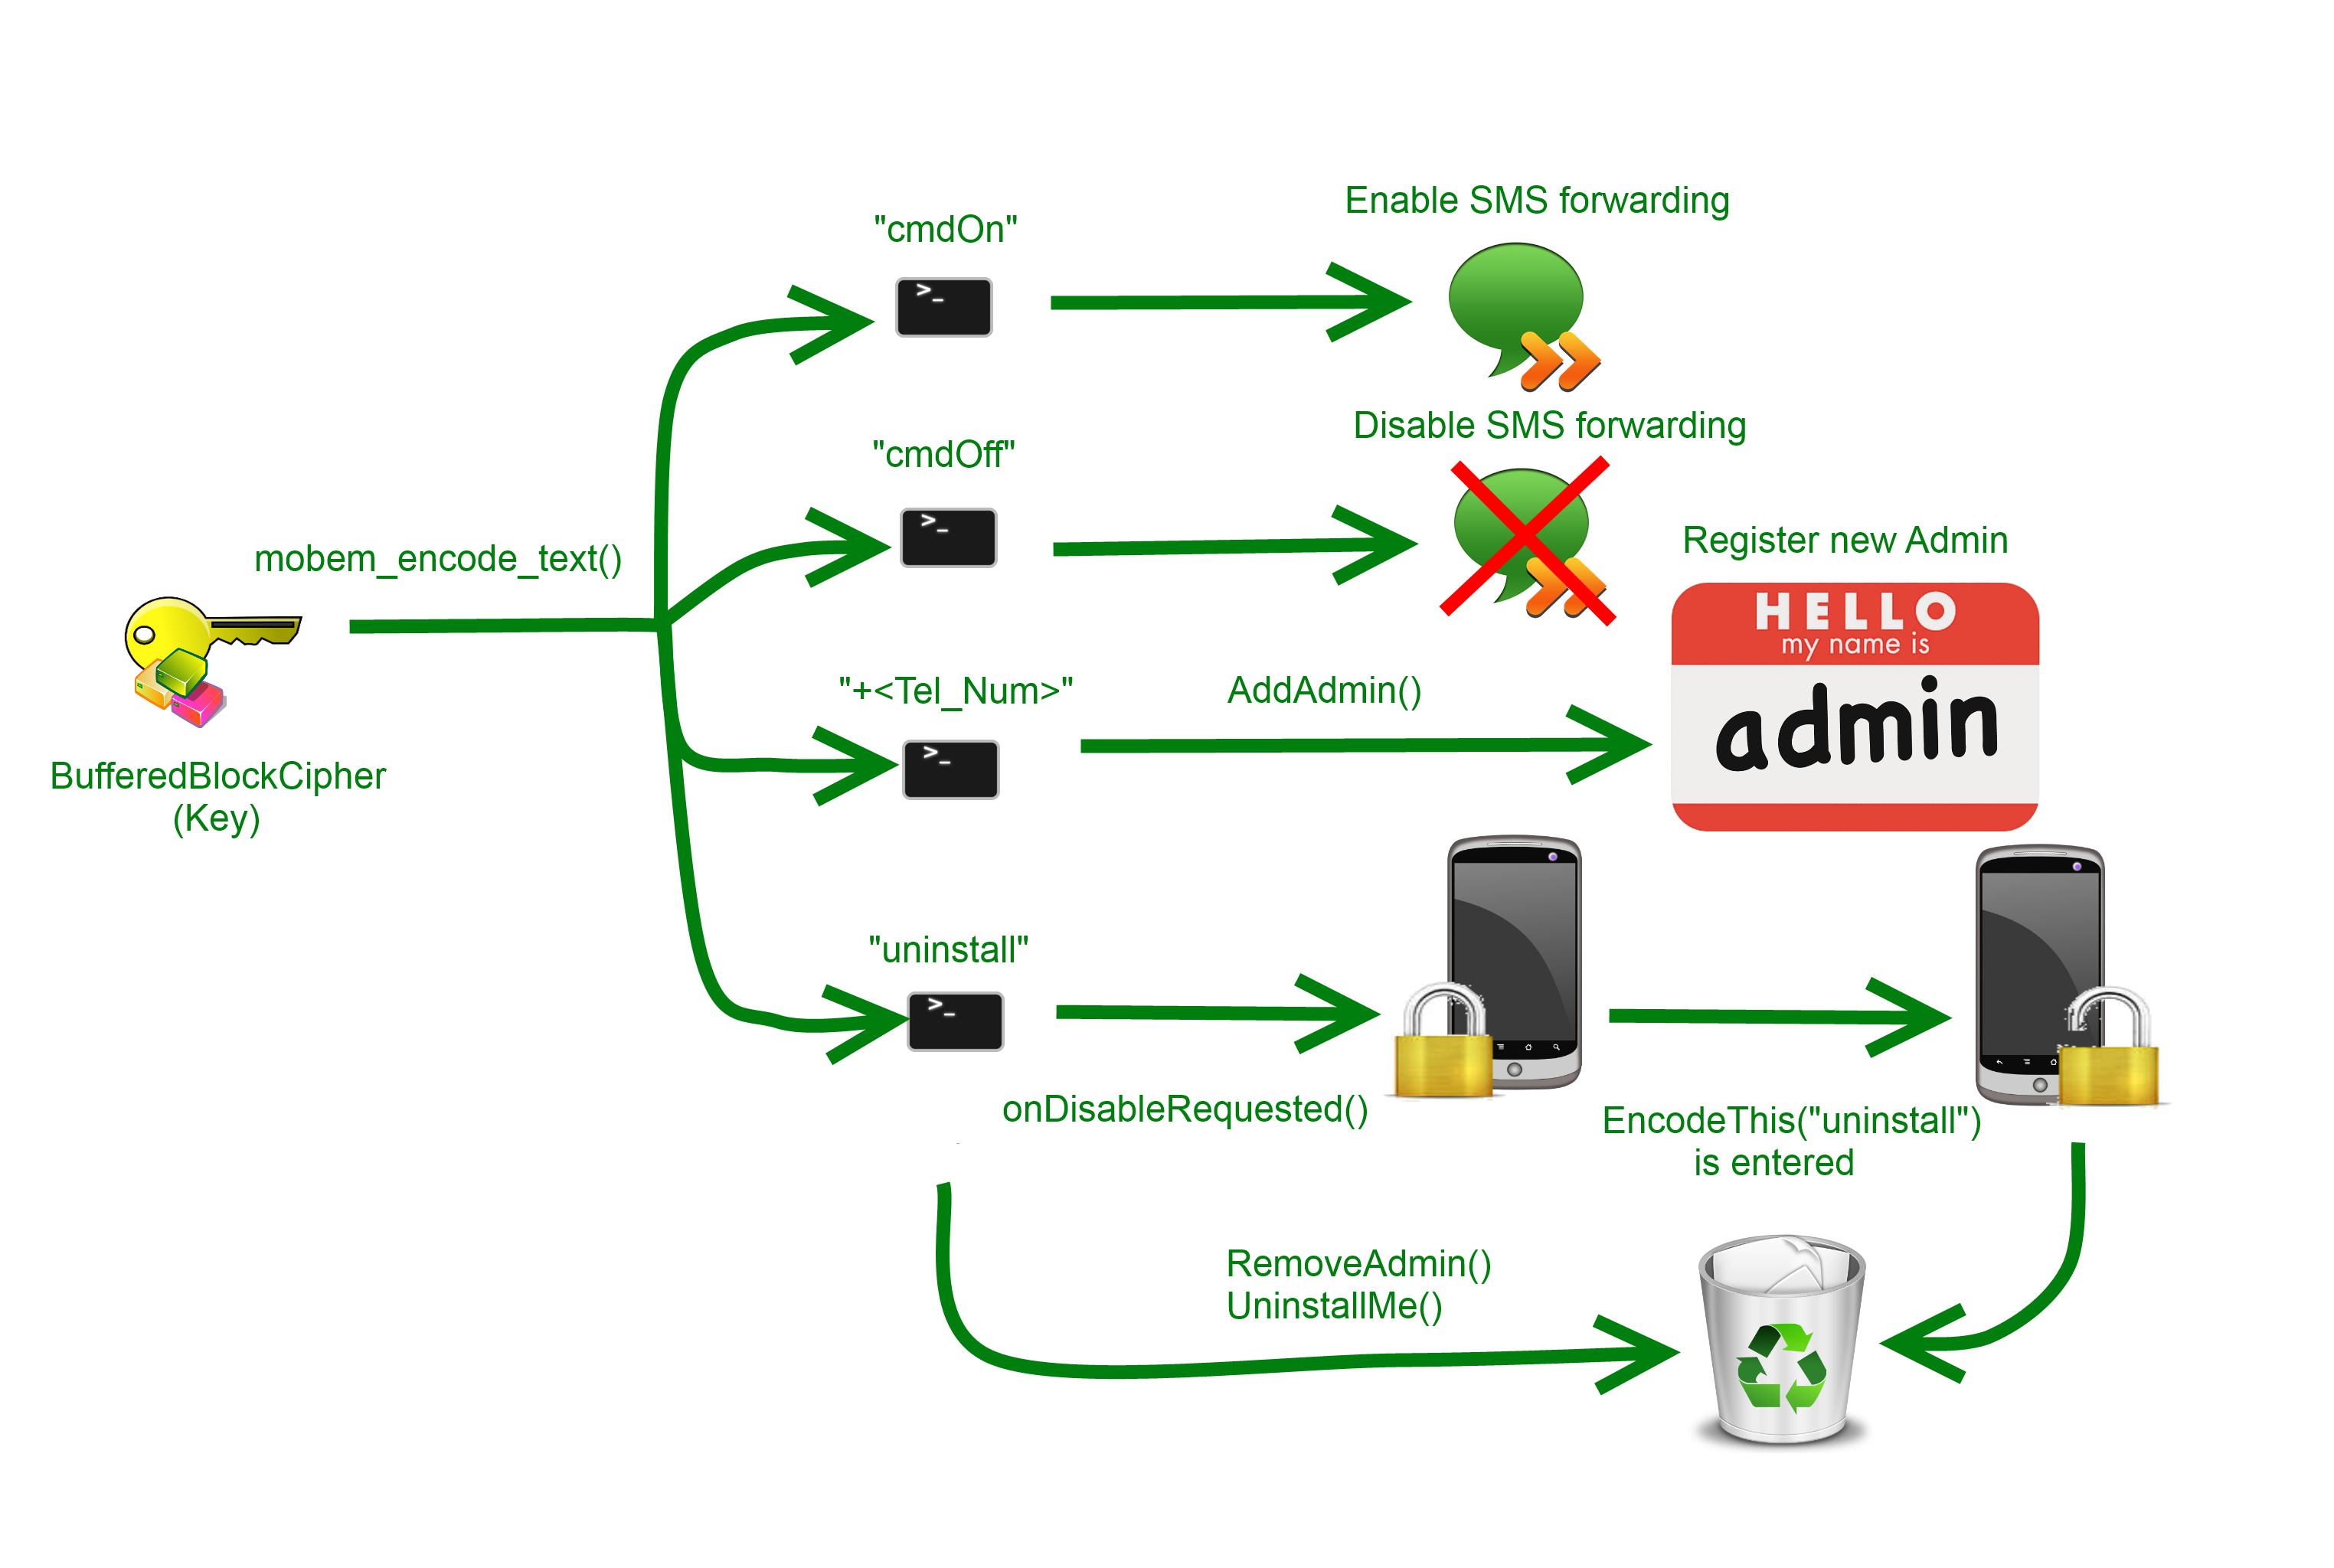
\includegraphics[height=0.9\textheight]{images/behaviour.png}
\end{frame}


\begin{frame}
\frametitle{Fake Login Screen}
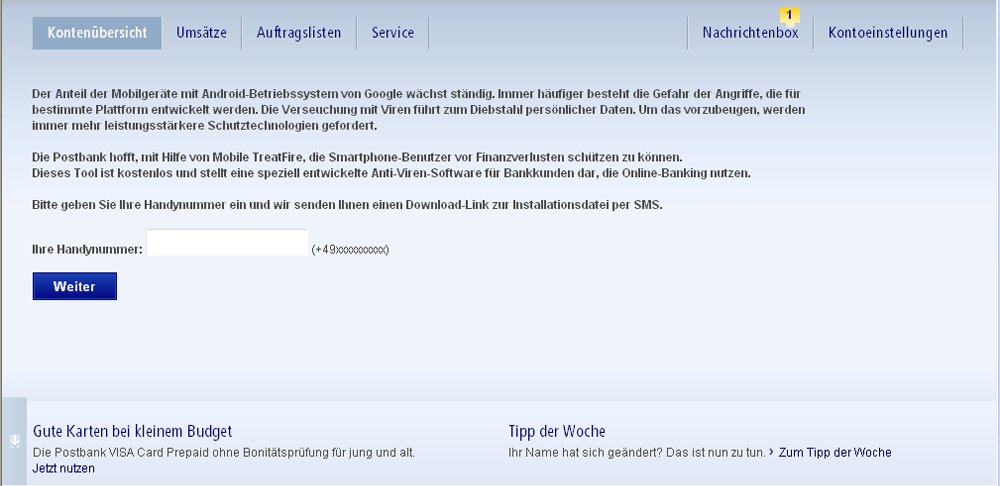
\includegraphics[width=\textwidth]{images/abfrage-der-rufnummer.png}
\blfootnote{Images from \url{http://www.postbank.de}}
\end{frame}

\begin{frame}
\frametitle{Fake Login Screen}
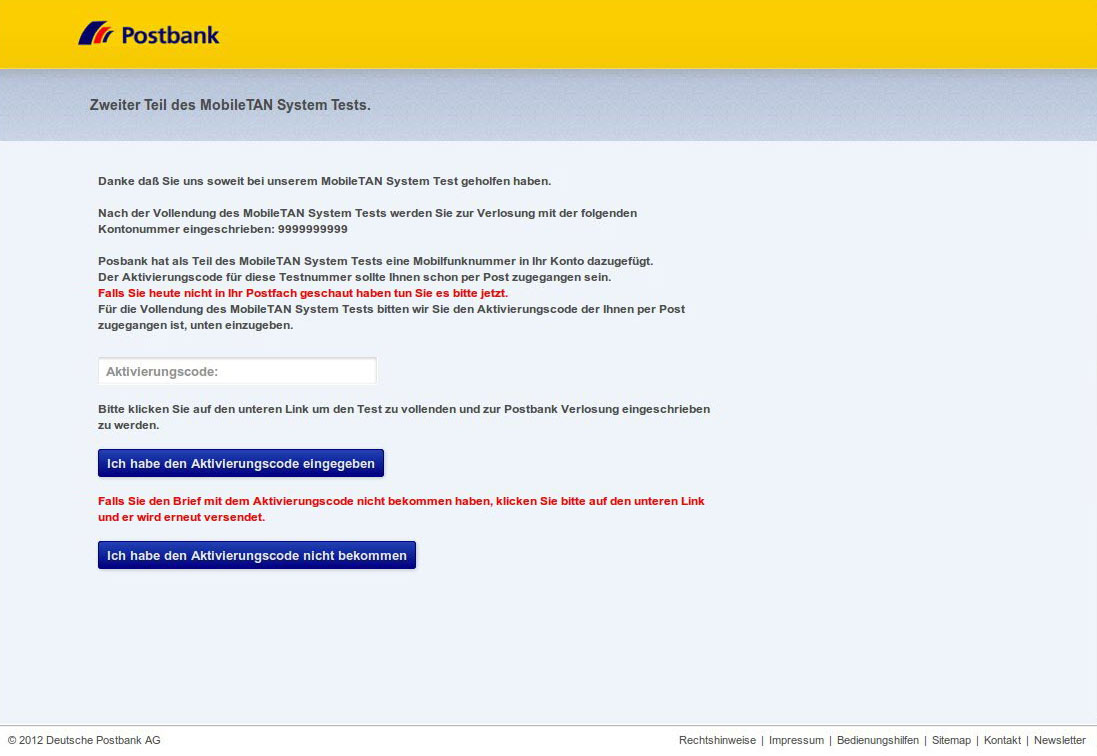
\includegraphics[width=\textwidth]{images/aktivierunsgcode-bank.jpg}
\end{frame}

\begin{frame}
\frametitle{Are there any other traps?}

\textbf{Answer}: Probably not ;)

\end{frame}

\section{Hacking}
\begin{frame}
\frametitle{What can we do?}
\begin{itemize}
	\item Rewrite as own Admin? No, activation code needed.
	\item Send uninstall Code? No, activation code needed.
	\item Decrypt Password? No, ...
	\item Conclusion: We need the activation or response code!
\end{itemize}

\end{frame}

\begin{frame}[fragile]
\frametitle{Abusing Malware}
Lets use reflection!

\begin{lstlisting}[style=customjava]
DexClassLoader dcl = new DexClassLoader(DEXPath,ODEXPath,null,this.getClassLoader());
Class<?> mycls = null;
mycls = dcl.loadClass("com.mobem.controller.mobem");
\end{lstlisting}

\end{frame}



\begin{frame}[fragile]
\frametitle{Abusing Malware}
Lets call some Methods!\\
For example: \texttt{public static boolean IN\_RANGE(int x, int a, int b)}
\begin{lstlisting}[style=customjava]
Method m = mycls.getMethod("IN_RANGE",int.class,int.class,int.class);

// 17 > 2 || 17 <16 => false
boolean r = (Boolean)m.invoke(null, 17,2,16); 
\end{lstlisting}

\end{frame}

\begin{frame}[fragile]
Generate all the things!
\begin{lstlisting}[style=customjava]
// loadCache will load a prepared cert.db file
Class <?> clsDatabaseAdapter = dcl.loadClass("com.certificate.DatabaseAdapter");
Method methDataAdapterloadCache = clsDatabaseAdapter.getMethod("loadCache");
Object localCache = methDataAdapterloadCache.invoke(instDatabaseAdapter);
// load the Encoder Method
Class <?> clsUtil = dcl.loadClass("com.certificate.Util");
Method encode = clsUtil.getDeclaredMethod("EncodeThis",String.class);

// generate Codes!
encode.invoke(null, "uninstall");
\end{lstlisting}

\end{frame}

{
\setbeamercolor{background canvas}{bg=bggrey}
\setbeamertemplate{background}{\parbox[c][\paperheight][c]{\paperwidth}{\centering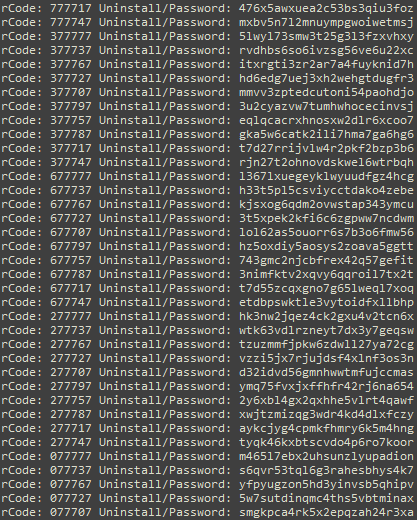
\includegraphics[height=\paperheight]{images/uninstallcodes.PNG}}}
\begin{frame}[plain]

\mybox{Generate all Codes!}

\end{frame}
}

\begin{frame}[fragile]
	\frametitle{The Response Code}
	Is well hidden in a \texttt{sqlite3} Database in \texttt{/data/data/com.certificate/databases/cert.db}
	\begin{itemize}
		\item Only Readable for the App and root
		\item We have no root nor the same group as the user
		\item \textbf{But} we can generate now codes from an existing DB!
	\end{itemize}
	
	\begin{lstlisting}[basicstyle=\tiny]
root@generic_x86:/data/data/com.certificate/databases # ls -al
ls -al
-rw-rw---- u0_a46   u0_a46      20480 2014-11-17 06:42 cert.db
-rw------- u0_a46   u0_a46      12824 2014-11-17 06:42 cert.db-journal
\end{lstlisting}
\end{frame}
{
\usebackgroundtemplate{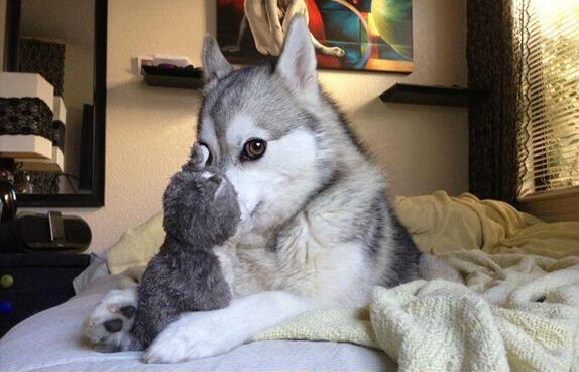
\includegraphics[height=\paperheight]{images/punhusky1.png}}
\begin{frame}[plain]
\raisebox{18em}{\mybox{Wait, what Android Version was it?}}
\end{frame}
}
{
\usebackgroundtemplate{
\includegraphics[width=\paperwidth]{images/punhusky3.png}}
\begin{frame}[plain]
\raisebox{-20em}{\mybox{Oh it's a Masterkey Exploitable 4.1!}}
\end{frame}
}

\begin{frame}
\frametitle{Master Key Exploit}
\begin{itemize}
	\item Different implementation of ZIP parser in Android
	(By the way ZIP is a weird format...)
	\item Duplicate items in ZIP will cause different outcomes
	\item Original classes.dex for verification
	\item \textbf{Our} classes.dex for execution! 
\end{itemize}
\end{frame}


\begin{frame}
\frametitle{Brainstorming}
\large
\centering
We need to get \texttt{rCode} and we need a trigger from outside...

\end{frame}

\begin{frame}[fragile]
\frametitle{Solution}
Use the SMS Receiver to execute our code in the Context of the Malware:
\begin{lstlisting}[style=customjava]
String db_path = "/data/data/com.certificate/databases/cert.db";
db = SQLiteDatabase.openDatabase(db_path, null, SQLiteDatabase.OPEN_READONLY);
db.rawQuery("select * from settings", null);
\end{lstlisting}

\end{frame}


\begin{frame}
\frametitle{One Problem left...}
\large
\centering
Where can we get a version of WinRAR that allows to pack duplicate filenames?

\end{frame}

\begin{frame}
\frametitle{One Problem solved!}
\large
\centering

Oh good! We never updated it!

\end{frame}


\begin{frame}
\frametitle{How to create a MKE APK}
\centering
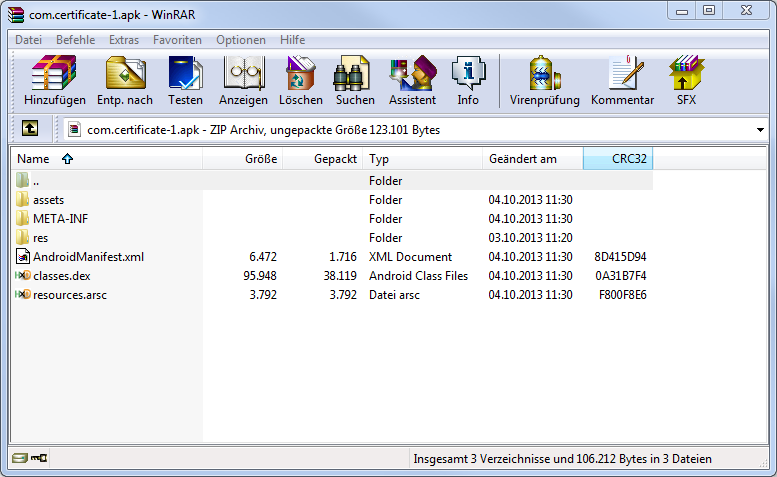
\includegraphics[width=\textwidth]{images/before-mke.png}
\end{frame}

\begin{frame}
\frametitle{How to create a MKE APK}
\centering
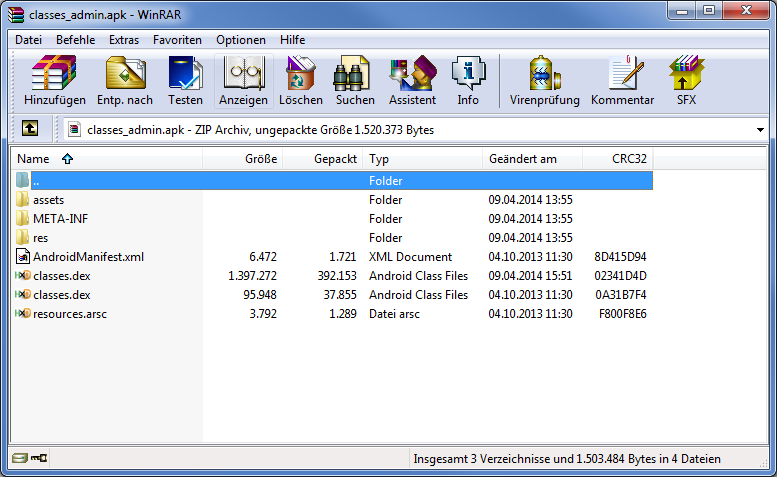
\includegraphics[width=\textwidth]{images/after-mke.png}
\end{frame}

\begin{frame}[fragile]
\frametitle{One Last Chance...}

\begin{lstlisting}
$ adb -r install exploited_apk.apk
\end{lstlisting}

adb logcat
\begin{lstlisting}
I/PackageManager(  389): Package com.certificate codePath changed from /data/app/com.certificate-1.apk to /data/app/com.certificate-2.apk; Retaining data and using new
\end{lstlisting}

\end{frame}


\begin{frame}[fragile]
\frametitle{Success!}

\begin{lstlisting}
E/mytag   ( 3075): rCode / 361484
E/mytag   ( 3075): admin / +380964123254
E/mytag   ( 3075): on / off
E/mytag   ( 3075): last_stamp / 1396939544764
\end{lstlisting}

\begin{itemize}
	\item Attacker used Ukrainian Telephone Number
	\item Last contact was at 2014-04-08 6:45:44 am CEST
	\item The Attacker disabled the trojan
	\item Uninstall Code translates to: \texttt{k3zp7iq4r6ggwktjrmt3jlxl3}
	\item Activation Code was: 899172
\end{itemize}

\end{frame}

\section{What we have learned}


{
\setbeamercolor{background canvas}{bg=simpsongreen}

\begin{frame}
\frametitle{\texttt{// TODO FIXME}}

\begin{itemize}
{\color{white}
	\item[] I will not remove malware until I analyzed it
	\item[] I will not remove malware until I analyzed it
	\item[] I will not remove malware until I analyzed it
	\item[] I will not remove malware until I analyzed it
	\item[] I will not remove malware until I analyzed it
	\item[] I will not remove malware until I analyzed it
	\item[] I will not ...
}
\end{itemize}

\begin{figure}
\hfill
\includegraphics[scale=0.4]{images/bart.png}

\end{figure}

\end{frame}
}



\begin{frame}
\frametitle{\texttt{// TODO FIXME}}
\begin{itemize}
	\item Follow Rules for Forensic Analysis (e.g. SANS) \footnote{\url{http://www.sans.org/reading-room/whitepapers/incident/computer-forensics-weve-incident-investigate-652}}
	\item Create a Checklist \& Ruleset for your internal use
	\item Assume the worst-case
	\item Build analysis tools to show you the dangerous stuff
	\item Try \textbf{not to} be too hasty
	\item Try to be as precise as possible!
	\item Do not start your analysis on friday afternoon ;)
\end{itemize}
\end{frame}

\begin{frame}
\frametitle{\texttt{// TODO FIXME}}
Dangerous activites are now highlighted
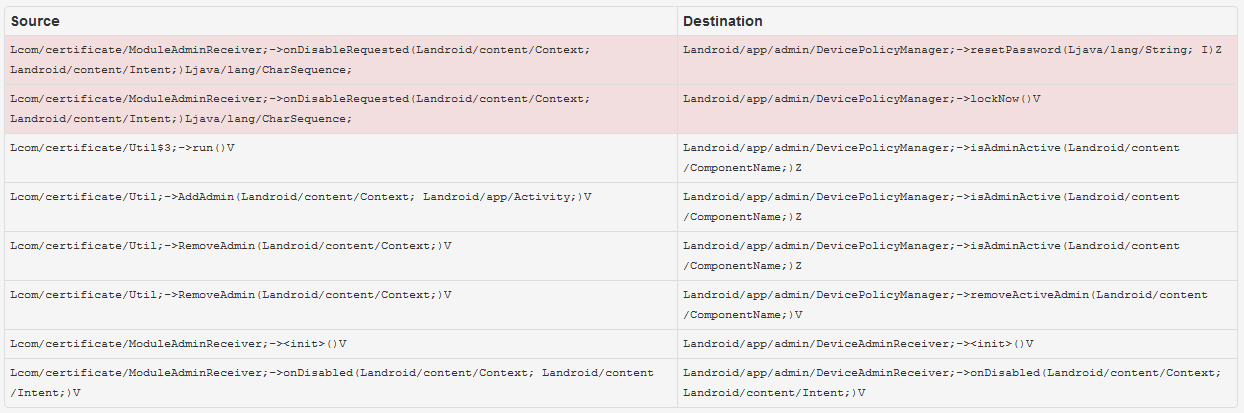
\includegraphics[width=\textwidth]{images/device-admin-analysis.png}


\end{frame}

\begin{frame}
\frametitle{\texttt{// TODO FIXME}}

\begin{itemize}
	\item Make Backups, even from your Smartphone
	\item If Ransomware hits you, just reset the device...
\end{itemize}

\end{frame}



\section{EOF}

\begin{frame}
\frametitle{EOF}

\centering
Source of Hesperbot Cracker\\
{\footnotesize (Including all Uninstall Codes)}
\small\url{https://github.com/IKARUSSoftwareSecurity/hesperbot-cracker}

\vspace{4em}

  \begin{columns}
    \begin{column}{.5\linewidth}
    \centering
	\textbf{Sebastian Bachmann}
	
	\vspace{1em}
	
	\url{https://www.reox.at}

	\vspace{1em}	
	
	bachmann.s@ikarus.at
    \end{column}
    \begin{column}{.5\linewidth}
    \centering
	\textbf{Tibor Éliás}
	
	\vspace{1em}
	
	\qquad

	\vspace{1em}	
	
	elias.t@ikarus.at
    \end{column}
  \end{columns}
\end{frame}


\end{document}